% Chapter X

\chapter{Poumon} % Chapter title


\label{ch:01-02} % For referencing the chapter elsewhere, use \autoref{ch:name} 

%----------------------------------------------------------------------------------------

% \section{}

A la suite de la trachée on à l’organe central de la respiration, le poumon qui est situé dans la cage thoracique au-dessus du diaphragme. Une double membrane séreuse, la plèvre pariétale, située contre la paroi thoracique et la plèvre viscérale maintien le poumon contre la paroi thoracique. \\
\\
Hors pathologies, l’Homme possède deux poumons séparés l’un de l’autre par le médiastin. Le poumon dit droit est divisé en trois lobes et le gauche en deux, ceci étant dû à la place occupée par le cœur. Chacun de ces lobes est relié à la trachée via une bronche souche qui se divise en bronches plus petites, puis en bronchioles à l’extrémité desquelles on retrouve les alvéoles regroupées par grappe, lieux principal des échanges gazeux entre l'air baignant les alvéoles et le sang des capillaires. (Figure \ref{poumon})

\begin{center}
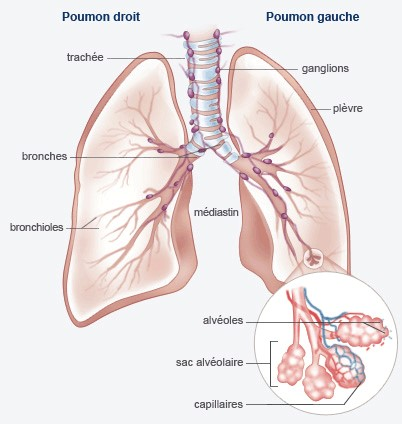
\includegraphics[scale=0.7]{gfx/poumon.jpg} 
\captionof{figure}{Poumon}
       \label{poumon}
\end{center}

		\section{Bronche et Bronchioles}
Les bronches primaires (ou souches) se divisent en bronches lobaires puis en bronches segmentaires pour finir par les bronchioles. D’architecture semblable à la trachée, les bronches primaires présentent un épithélium de type respiratoire identique à celui de la trachée mais aussi quelques différences: une discontinuité des anneaux cartilagineux, elles présentent également un réseau de fibres élastiques plus important dans le chorion qui fait office de séparation avec la sous muqueuse qui contient moins de structures glandulaires.\\
\\
Les bronchioles sont très fines (0.5 à 1mm de diamètre) divisées en trois types chacun étant progressivement de plus en plus petit : les bronchioles lobaires, les bronchioles terminales et les bronchioles respiratoires. Il n’y a pas d’échange d’air dans les bronchioles lobaire et terminales par contre on a un échange au niveau des bronchioles respiratoire. La fonction primaire des bronchioles est de conduire l’air des bronches aux alvéoles et de contrôler le débit d’air distribué dans le poumon par constriction ou dilatation. \\
\\
La structure des bronchioles est sensiblement différente des celles des bronches. Alors que les bronches sont entourées d’un anneau de cartilage qui permet de les maintenir ouvert, les bronchioles sont-elles entourées d’un mur de muscle lisse permettant de dilater et de contracter les voies respiratoires contrôlant ainsi la livraison d’air aux alvéoles. Leur muqueuse est formée d’un épithélium simple cylindrique dépourvu de cellules caliciformes et pauvre en cellules ciliées. Le chorion est réduit à une fine lame élastique et la sous muqueuse qui se confond avec l’adventice ne contient pas de glandes. (Figure\ref{bronche})

\begin{center}
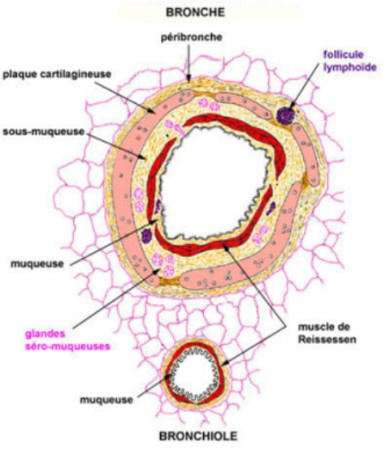
\includegraphics[scale=1.6]{gfx/bronche.jpg} 
\captionof{figure}{Bronche}
       \label{bronche}
\end{center}


		\section{Alvéoles}
A l’aboutissement de l’arbre bronchique on retrouve les alvéoles regroupées en acinus pulmonaire. Un acinus est constitué des 5 à 6 alvéoles entourées d’un réseau de capillaire sanguin fixé et intiment lié à la fonction des alvéoles.\\
\\
L’épithélium alvéolaire est constitué de pneumocytes de deux types différents type I (membraneux) et type II (granuleux). La barrière alvéolo-capillaire au travers de laquelle est assuré la fonction d’échanges gazeux est formée des Pneumocytes de type I des alvéoles et des cellules endothéliales des capillaires. \\
\\
Alors que la proportion en Pneumocytes I et II est sensiblement identique, les Pneumocytes de type I, du fait de leurs structures fines (0,1 à {0,2}{\micro\metre} d'épaisseur) et étalées, couvrent 95\% de la surface alvéolaire. Ceci a pour conséquence de conférer à l’épithélium alvéolaire une caractéristique souple très étendu qui favorise les échanges gazeux, mais aussi très fragile qui le rend vulnérable aux attaques microbiennes et aux polluants.\\
\\
Les pneumocytes de type II sont de forme cubique et présente une microvillosité au niveau de leurs pôle apical. Leurs aspect granuleux est dû à leur cytoplasme riche en organites dont un spécifique, les corps lamellaires qui sécrètent le surfactant pulmonaire, de plus ils présentent un réticulum endoplasmique et un appareil de Golgi surdéveloppés signe d’un métabolisme très actif. \\
Le surfactant sécrété (et aussi recyclé), par les corps lamellaires des pneumocytes de type II, a pour fonction de fluidifier le mucus et de facilite les échanges gazeux, de diminuer la tension de surface des alvéoles afin qu'elles ne s'effondrent pas sur elles-mêmes pendant la respiration et à la conservation de l'élasticité des poumons. (Figure \ref{alveol})


\begin{center}
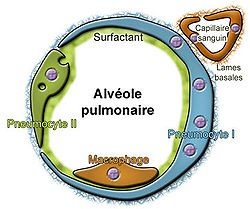
\includegraphics[scale=0.7]{gfx/alveole.jpg} 
\captionof{figure}{Alvéole}
       \label{alveol}
\end{center}

		\section{Pathologies}
Les maladies pulmonaires ont essentiellement des causes infectieuses (bactéries, virus ou champignons pathogènes). Le plus fréquent étant le pneumocoque (Streptococcus pneumoniae) qui est aussi l’un des plus dangereux. \\
Parmi les pathologies pulmonaires fréquentes on trouve l’asthme, les bronchopneumopathies chroniques obstructives (BCPO) caractérisé par un rétrécissement irréversible des bronches, cancers et la mucoviscidose maladie génétique caractérisé par une production importante d’un mucus épais qui entraîne d’important troubles respiratoires. On peut en citer pleins d’autre mais c’est sur cette dernière pathologie que notre étude se concentre.




%------------------------------------------------

% \subsection{Subsection Title}

% Content